\documentclass[b5paper,opensource]{./template/qyxf-book}
%,sourcefont,parskip
%\usepackage{subcaption}
%\usepackage{draftwatermark}
%\usepackage{fontawesome5}
%\SetWatermarkText{钱院学辅}
%\SetWatermarkLightness{0.92}
%\SetWatermarkScale{0.9}

\usepackage{siunitx}%输入角度
\usepackage{color}
\renewcommand{\thefootnote}{\color{red}\arabic{footnote}}%更改脚注格式
%\newcommand{\tabincell}[2]{\begin{tabular}{@{}#1@{}}#2\end{tabular}}%单元格内强制换行
\usepackage{subfigure}%并排图片
%\renewcommand{\figurename}{图}
%\renewcommand{\thefigure}{}
%如何去掉子图下面的标注(a)?从代码中把 \subfigure[]的中括号去掉即可。
\usepackage{float}%图片插入在文字右侧,\begin{figure}[H]尝试失败
%这里面有很多图片被迫转到下一页的,还有就是无法环绕文字,即图题分离,造成麻烦,怎么办?
\usepackage{CJKfntef}%文字下加点

\newcommand{\di}[1]{\mathrm{d}#1}%微分
\newcommand{\p}[2]{\dfrac{\partial #1}{\partial #2}}
\newcommand{\pp}[2]{\dfrac{\partial ^2 #1}{\partial #2 ^2}}
\newcommand{\dy}[2]{\dfrac{\di{#1}}{\di{#2}}}
\newcommand{\ddy}[2]{\dfrac{\mathrm{d} ^2 #1}{\mathrm{d} #2 ^2}}
\newcommand{\zbj}[4]
{
	\draw (0,0) node[below left] {$ O $};
	\draw [->] (#1,0) -- (#2,0) node[right] {$ x $};
	\draw [->] (0,#3) -- (0,#4) node[right] {$ y $};
}
\newcommand{\tips}{\noindent\textbf{提示}\ }
\RequirePackage{tabularx}%改变表格宽度
%下面新定义了几个选项的样式
\newcommand{\option}[4]{
	\begin{center}
		\begin{tabularx}{\textwidth}{*{4}{>{\arraybackslash}X}}
			\tcbox[on line,top=0mm,bottom=0mm,right=0mm,left=0mm]{\bfseries A.} $#1$&
			\tcbox[on line,top=0mm,bottom=0mm,right=0mm,left=0mm]{\bfseries B.} $#2$&
			\tcbox[on line,top=0mm,bottom=0mm,right=0mm,left=0mm]{\bfseries C.} $#3$&
			\tcbox[on line,top=0mm,bottom=0mm,right=0mm,left=0mm]{\bfseries D.} $#4$
		\end{tabularx}
	\end{center}
}%选项,横排1*4
\newcommand{\options}[4]{\\
	\begin{tabularx}{\textwidth}{*{1}{>{\arraybackslash}X}}
		\tcbox[on line,top=0mm,bottom=0mm,right=0mm,left=0mm]{\bfseries A.} #1\\
		\tcbox[on line,top=0mm,bottom=0mm,right=0mm,left=0mm]{\bfseries B.} #2\\
		\tcbox[on line,top=0mm,bottom=0mm,right=0mm,left=0mm]{\bfseries C.} #3\\
		\tcbox[on line,top=0mm,bottom=0mm,right=0mm,left=0mm]{\bfseries D.} #4
	\end{tabularx}
}%选项,竖排4*1
\RequirePackage{siunitx}
%\renewcommand{\arraystretch}{2}%调整矩阵行间距,这本来应该调行距的,但我没成功
%{l@{\extracolsep{\fill}}l}
\newcommand{\optionss}[4]{
	\renewcommand{\arraystretch}{1.5}%调整表格行间距
	\begin{center}
		\begin{tabularx}{\textwidth}{*{2}{>{\arraybackslash}X}}
			\linespread{2}
			\tcbox[on line,top=0mm,bottom=0mm,right=0mm,left=0mm]{\bfseries A.} $#1$&
			\tcbox[on line,top=0mm,bottom=0mm,right=0mm,left=0mm]{\bfseries B.} $#2$\\
			\tcbox[on line,top=0mm,bottom=0mm,right=0mm,left=0mm]{\bfseries C.} $#3$&
			\tcbox[on line,top=0mm,bottom=0mm,right=0mm,left=0mm]{\bfseries D.} $#4$
		\end{tabularx}
	\end{center}
}%选项,横排2*2
\newcommand{\ul}{\underline{\quad\quad\quad\quad\quad\quad}}%填空题的下划线
\newcommand{\ull}{\underline{\quad\quad\quad\quad\quad\quad\quad\quad\quad}}%加长版
\newcommand{\choosing}[2]{\noindent\tcbox[on line,top=0mm,bottom=0mm,right=0mm,left=0mm]{\bfseries 选择#1$\sim$#2}\ }%选择题答案
\newcommand{\filling}[8]{
	\renewcommand{\arraystretch}{1.6}%调整表格行间距
	\begin{tabularx}{\textwidth}{*{1}{>{\arraybackslash}X}}
		\noindent\leftline{\tcbox[on line,top=0mm,bottom=0mm,right=0mm,left=0mm]{\bfseries 填空1} $#1$}\\
		\noindent\leftline{\tcbox[on line,top=0mm,bottom=0mm,right=0mm,left=0mm]{\bfseries 填空2} $#2$}\\
		\noindent\leftline{\tcbox[on line,top=0mm,bottom=0mm,right=0mm,left=0mm]{\bfseries 填空3} $#3$}\\
		\noindent\leftline{\tcbox[on line,top=0mm,bottom=0mm,right=0mm,left=0mm]{\bfseries 填空4} $#4$}\\
		\noindent\leftline{\tcbox[on line,top=0mm,bottom=0mm,right=0mm,left=0mm]{\bfseries 填空5} $#5$}\\
		\noindent\leftline{\tcbox[on line,top=0mm,bottom=0mm,right=0mm,left=0mm]{\bfseries 填空6} $#6$}\\
		\noindent\leftline{\tcbox[on line,top=0mm,bottom=0mm,right=0mm,left=0mm]{\bfseries 填空7} $#7$}\\
		\noindent\leftline{\tcbox[on line,top=0mm,bottom=0mm,right=0mm,left=0mm]{\bfseries 填空8} $#8$}
	\end{tabularx}
}%填空题答案
\newcommand{\exerciseanswer}[2]{\noindent\tcbox[on line,top=0mm,bottom=0mm,right=0mm,left=0mm]{\bfseries #1#2}\ }%选填解析
\newcommand{\exercisequestion}[1]{\quad\tcbox[on line,top=0mm,bottom=0mm,right=0mm,left=0mm]{\bfseries (#1)}\ }%解答题号
\newcommand{\solves}[1]{\exercise{#1}\\ \solve}%解答题题头
\newcommand{\amperecircuitaltheorem}[1]{在距离电流$r$处,取一半径为$r$的环路,由安培环路定理:
	\begin{gather*}
	B\cdot 2\pi r=\mu_0I_{#1}\\
	B=\dfrac{\mu_0I_{#1}}{2\pi r}
	\end{gather*}
}
%\renewcommand{\sqrt}{\sqrt[\uproot{12}]}算了,在文中用吧


\title{大学物理往年期末试题(上)}
\subtitle{Key to Previous Final Tests of University Physics: Part I}
\author{钱院学辅大物编写小组}
\typo{钱院学辅排版组}
%\date{2019 年 6 月 9 日}
\version{v1.0}
\sourcepage{\url{https://github.com/qyxf/BookHub/}}

%本资料目前仅限钱学森书院内部使用
%图片的大小和位置还请排版组调一下,很多需要换页不方便,如果能放在题目右侧也行
%物体名和点未用斜体
%看到用\big调大小的就帮我改成\left吧

%\exercise,\note,\solve,\analysis,\tips提示
%\option,\options,\optionss(数学环境):选项排版
%\choosing{1}{10}:选择题答案
%\filling:填空题答案
%\exerciseanswer选填解析
%\exercisequestion解答题号
%\solves解答题题头
%\amperecircuitaltheorem 由安培环路定理,参数是I的下标

\begin{document}
\maketitle
\pagestyle{plain}
\chapter*{前言}%简单说一下
在排版这套资料之前,笔者刚刚经历大学物理上的期末考试,做了一些往年的试题。但市面上流通的资料有太多错漏,这让笔者颇为恼火。为了让学弟学妹们少遇到一些麻烦,笔者才产生了重新排版往年题的想法。本题册中,部分原版中的错误已经被改正,有的题目也进行了修改。这些修改以促进使用者思考、培养使用者思路为目的,并不再在题册中标注。

2017年以后(我不确定时间),我校开始实行大学物理两次阶段测试和一次期末考试的制度,这期间的考试真题大多没有拿在同学们的手上;2014$\sim$2016年考察的内容与现在不同(应该是大学物理下);2012年之前的题与现在考察的内容相似。不过2019年的题中,选择题10$\times$3,填空题改成了简答题(4$\times$5),形式类似于解答题(5$\times$10),但比真正的解答题或填空题简单很多(怕是想给大家加分……)。2019年的考试题很简单,考察的也多是简单概念,没有用什么高超的技巧。这毕竟不是竞赛,而且会做许多难的物理题在大学也用处不大。如果成绩好,笔者建议参加大学物理研讨班,(尽管笔者的专业是化生试验班)它培养了一种解决问题的方法,对我们更加有用,还有成绩加成。

根据徐忠锋老师的说法,我校大学物理只是一门“通识课”,重在体会其思想,并不建议大家做很多题;再者,考试题目难度本身就低于作业题,考前看一遍课本,过一遍作业题(欢迎大家参考钱院学辅出版的《大学物理题解》系列),其价值更高,对付考试没有问题;其三,作业题一直在更新,比起多年前的考试题更有参考价值。只是说,对于考前才突击和考前心里没底、想找感觉的同学,往年题才有一定的作用。如果先做了这些题,最好再看看老师提供的复习提纲(知识框架),找找遗漏的点(比如,静电平衡的性质,不起眼但很致命);做题时,回溯课本也往往能找到某些想要的答案。

%为了给使用者充分的自由,我们建议使用者自己找一张纸,或利用题册的背面来作答。
电子版使用者可以打开PDF阅读器的目录,方便跳转到答案;对于纸质版使用者,我们将题目答案设在每章的后面,以方便查看,也避免误看到下一章的答案。

由于题目难度不大,我们只给出所有更正后的答案和部分题目解析,如还有问题,欢迎各位使用者来钱学森书院三楼自习室答疑。限于笔者水平,笔误、错漏等在所难免,给使用者带来的不便敬请谅解,也恳请各位使用者帮助我们指正。

如果有近年的试题流出,我们也将尽快整理出来供大家使用。
\vspace{2em}

\begin{flushright}
	高旭帆
\end{flushright}
\vspace{1.0cm}
\begin{figure}[!h]
	\centering
	\begin{minipage}[c]{0.5\textwidth}
		\centering
		
\includegraphics[scale=0.5]{./template/qrcode2.png}
	\end{minipage}%
	\begin{minipage}[c]{0.5\textwidth}
		\centering
		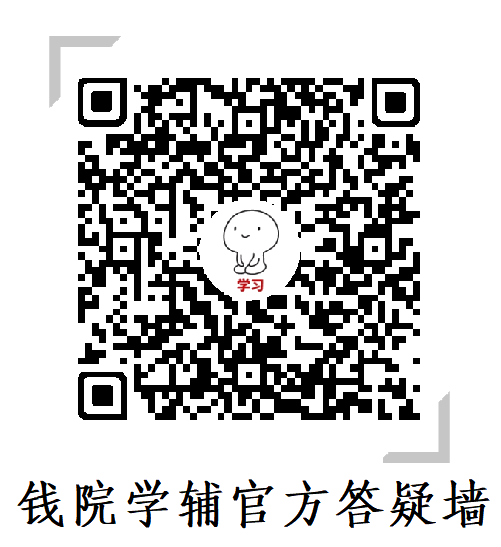
\includegraphics[scale=0.5]{./template/qxf.png}
	\end{minipage}
\end{figure}



\newpage
\tableofcontents
\setlength{\parindent}{0pt}
\chapter{2012年期末试题}
\section{选择题}
\exercise{1}
质点以速度$v=4+t^2 m/s$作直线运动,沿质点运动直线作OX轴,并已知$t=3$s时,质点位于$x=9$m处,则该质点的运动学方程为:
\optionss{x=3t}
{x=4t+\dfrac{1}{2}t^2}
{x=4t+\dfrac{1}{3}t^3-12}
{x=4t+\dfrac{1}{3}t^3+12}

\exercise{2}
力$\vec{F}=3\vec{i}+5\vec{J}$(N),其作用点的位置矢量为$\vec{r}=4\vec{i}-3\vec{j}$(m),则该力对坐标原点
的力矩大小为:
\option{3\textrm{N/m}}{29\textrm{N/m}}{19\textrm{N/m}}{3\textrm{N/m}}

\exercise{3}一特殊弹簧,弹性力 $F=-kx^3$,$k$为劲度系数,$x$为形变量。现将弹簧水平放置于光滑的平面上,一端固定,一端与质量为$m$的滑块相连而处于自然状态,今沿弹簧长度方向给滑块一个冲量,使其获得一速度$v$,则弹簧压缩的最大长度为:
\option{{{\left(\dfrac{4mv}{k}\right)}^{\frac{1}{4}}}}
{{\left(\dfrac{2mv^2}{k}\right)}^{\frac{1}{4}}}
{v\sqrt{\dfrac{k}{m}}}
{v\sqrt{\dfrac{m}{k}}}

\exercise{4}
一根质量为$m$,长为$l$的细而均匀的棒,其下端绞接在水平地板上并竖直的立起,如让它掉下(如图1.1a),则棒将以角速度$ω$撞击地板,如果将同样的棒截成长为$\dfrac{l}{2}$的一段,初始条件不变,则它撞击地板时的角速度最接近于
\option{2\omega}
{\sqrt{2}\omega}
{\omega}
{\frac{\omega}{\sqrt{2}}}
\begin{figure}[!h]
	\centering
	\subfigure[选择4 示意图]{
	\begin{minipage}[t]{0.3\linewidth}
		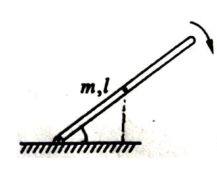
\includegraphics[width=\textwidth]{2012_1.png}
	\end{minipage}}
	\quad
	\subfigure[选择8 示意图]{
		\begin{minipage}[t]{0.3\linewidth}
		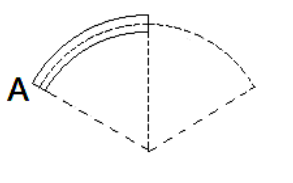
\includegraphics[width=\textwidth]{2012_2.png}
	\end{minipage}}
	\quad
	\subfigure[选择9 示意图]{
	\begin{minipage}[t]{0.3\linewidth}
		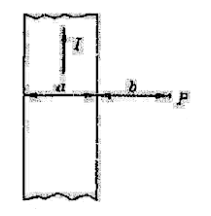
\includegraphics[width=\textwidth]{2012_3.png}
	\end{minipage}}
	\caption{三张题图}
\end{figure}
\exercise{5}
关于狭义相对论,下列几种说法中叙述\CJKunderdot{错误}的是:
\options{一切运动物体的速度都不能大于真空中的光速}
{在任何惯性系中,光在真空中沿任何方向的传播速率都相同}
{在真空中,光的速度与光源的运动状态无关}
{在真空中,光的速度与光的频率有关}

\exercise{6}两个均匀带电的同心球面,半径分别为$R_1,R_2(R_1<R_2)$,小球面带电$Q$,大球面带电$-Q$,下列各图中正确表示了电场分布的是
\begin{figure}[!h]
	\centering
	\option
	{\subfigure{
		\begin{minipage}[t]{\linewidth}
			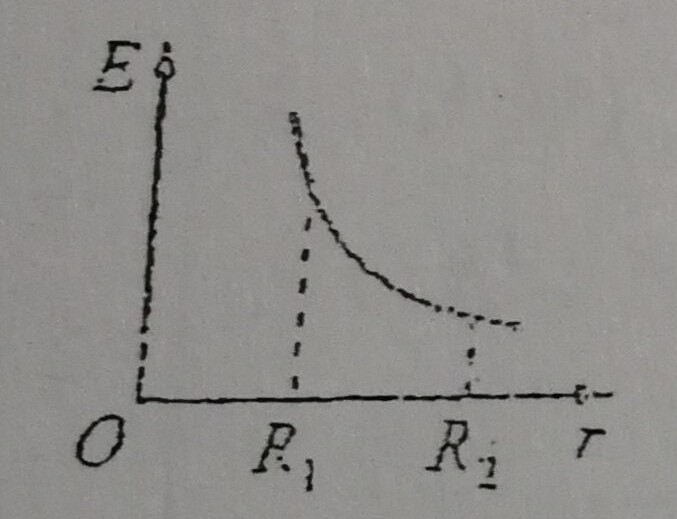
\includegraphics[width=\textwidth]{2012_4a.jpg}
	\end{minipage}}}
	{\subfigure{
		\begin{minipage}[t]{\linewidth}
			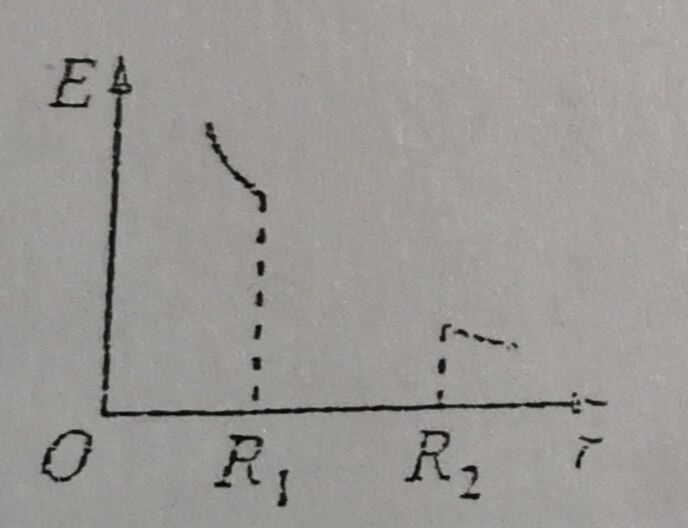
\includegraphics[width=\textwidth]{2012_4b.jpg}
	\end{minipage}}}
	{\subfigure{
		\begin{minipage}[t]{\linewidth}
			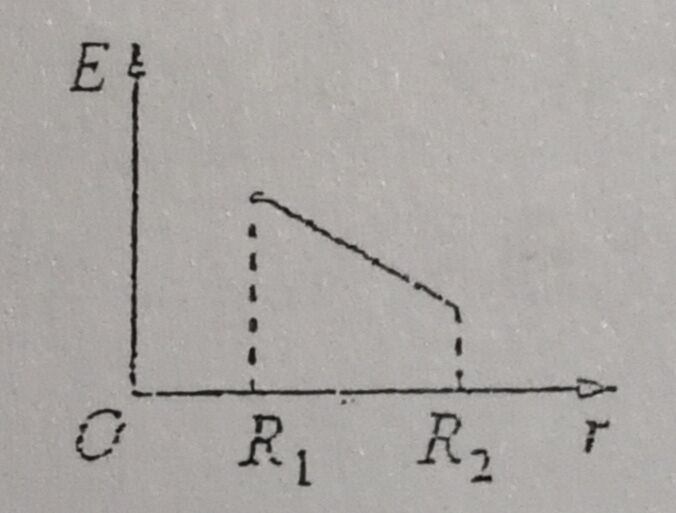
\includegraphics[width=\textwidth]{2012_4c.jpg}
	\end{minipage}}}
	{\subfigure{
	\begin{minipage}[t]{\linewidth}
		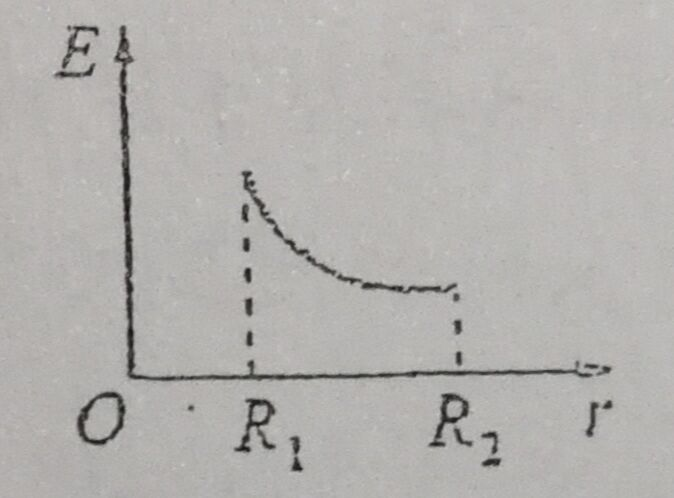
\includegraphics[width=\textwidth]{2012_4d.jpg}
	\end{minipage}}}
	\caption{选择6}
\end{figure}

\exercise{7}
磁场的高斯定理$\oiint\vec{B}\cdot\vec{S}=0$说明了下面表述正确的是:
\options{穿入闭合曲面$S$的磁感应线条数必然等于穿出的磁感应线条数}{穿入闭合曲面$S$的磁感应线条数不等于穿出的磁感应线条数}{一根磁感应线可以终止在闭合曲面$S$内}{一根磁感应线不可能完全处于闭合曲面$S$内}

\exercise{8}
有一均匀带电的绝缘体细圆弧,其圆心角为$\dfrac{2}{3}\pi$,测得其圆心$O$处的电场强度大小为$E_0$,今将此圆弧对折,如图,则$O$点电场强度大小为
\option{\dfrac{E_0}{2}}
{2E_0}
{\dfrac{\sqrt{3}}{3}E_0}
{\dfrac{2\sqrt{3}}{3}E_0}        

\exercise{9}
如图所示,有一无限长通有电流的薄平直铜片,宽度为$a$,厚度不计,电流$I$在铜片上均匀分布,在铜片外与铜片共面,离铜片右边缘为$b$处的$P$点的磁感应强度$\vec{B}$大小为
\optionss{\dfrac{\mu_0I}{2\pi(a+b)}}
{\dfrac{\mu_0I}{2\pi a}\ln\dfrac{a+b}{b}}
{\dfrac{\mu_0I}{2\pi b}\ln\dfrac{a+b}{a}}
{\dfrac{\mu_0I}{2\pi(\frac{a}{2}+b)}}%此处原题处多了个a

\exercise{10}
对位移电流,有下列四种说法,请指出哪一种说法正确
\options{位移电流是由变化的电场产生的\footnote{笔者认为此处说法不准确,应是“位移电流是变化的电场的一种等效”。详见参考答案。}}
{位移电流是由线性变化的磁场产生的}
{位移电流产生焦耳热}
{位移电流的磁效应不服从安培环路定理}

\section{填空题}

\exercise{1}
质量为$m$的物体,初速极小,在外力作用下从原点起沿x轴正向运动,所受外力方向沿x轴正向,大小为$F=kx$。物体从原点运动到坐标为$x_0$点的过程中所受外力冲量的大小为\ul。
%为什么初速极小

\exercise{2}
如图所示,一条轻质细绳绕过一个半径为$R$,转动惯量为$mR^2$的定滑轮(轮轴光滑),一端系着一个质量为 $2m$的物体,另一端有质量为$4m$的人抓住绳子相对于绳子匀速向上爬,则物体的加速度大小为\ul;若人相对于地面匀速向上爬,则物体的加速度大小为\ul。
\begin{figure}[!h]
	\centering
	\subfigure[填空2 示意图]{
		\begin{minipage}[t]{0.3\linewidth}
			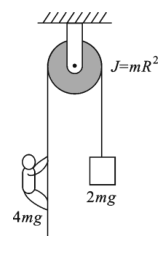
\includegraphics[width=\textwidth]{2012_5.png}
	\end{minipage}}
	\quad
	\subfigure[填空5 示意图]{
		\begin{minipage}[t]{0.5\linewidth}
			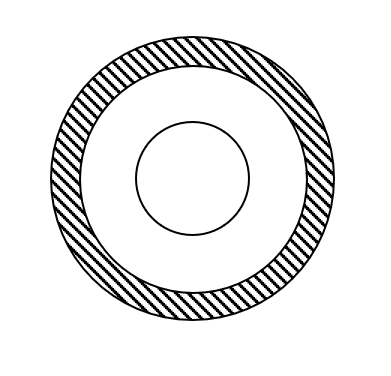
\includegraphics[width=\textwidth]{2012_6.ai}
	\end{minipage}}
	\caption{两张题图}
\end{figure}

\exercise{3}
一个人站在转动的转台中央,在他伸出的两个手中各握有一个重物,若此人向着胸部缩回他的双手及重物,忽略所有摩擦,则系统的转动惯量\ul,系统的转动角速度\ul,系统的角动量\ul ,系统的转动动能\ul。(填增大、减小或不变)

\exercise{4}
设电子的静止质量为$m_0$,将一个电子从静止加速到速率为$0.6c$($c$为真空中光速),需做功\ul。在速度$v=$\ul 的情况下电子的动能等于它的静止能量。

\exercise{5}
如图所示,一带电荷量为$q$,半径为$r_A$的金属球$A$,与一原先不带电、内外半径分别为$r_B$和$r_C$的金属球壳$B$同心放置。则图中$P$点的电场强度大小$E=$\ul。如果用导线将$A,B$连接起来,则$A$球的电势 $U=$\ul。(设无穷远处电势为零)

\exercise{6}
两块无限大的均匀带电平行平板,其电荷面密度分别为$\sigma$及$-2\sigma$,如图所示,试写出各区域的电场强度$\vec{E}$的大小:1区$\vec{E}$的大小\ul;2区$\vec{E}$的大小\ul;3区$\vec{E}$的大小\ul。

\exercise{7}
同种材质、粗细均匀的载流导线在平面内分布,弯成如图所示形状。导线中通有电流为$I,I_1,I_2$。它们在点$O$的磁感应强度\CJKunderdot{大小}为(用含$I_1,I_2$的式子表示)\ul;代入$I_1,I_2$大小关系可得磁感应强度大小为\ul。

\begin{figure}[!h]
	\centering
	\subfigure[填空6 示意图]{
		\begin{minipage}[t]{0.3\linewidth}
			\includegraphics[width=\textwidth]{2012_7.ai}
	\end{minipage}}
	\quad
	\subfigure[填空7 示意图]{
		\begin{minipage}[t]{0.3\linewidth}
			\includegraphics[width=\textwidth]{2012_8.ai}
	\end{minipage}}
	\quad
	\subfigure[填空8 示意图]{
		\begin{minipage}[t]{0.3\linewidth}
			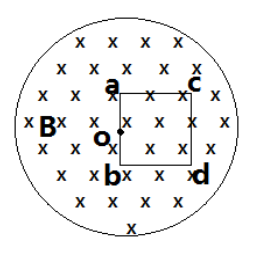
\includegraphics[width=\textwidth]{2012_9.png}
	\end{minipage}}
	\caption{三张题图}
\end{figure}

\exercise{8}
圆柱形区域内存在一匀强磁场$B$,且以恒定变化率$\dy{B}{t}$减小,一边长为$l$的正方形导体框abcd置于该磁场中,框平面与磁场垂直,圆柱形匀强磁场中心O位于ab的中心,如图所示,则c处有旋电场强度大小$E_c=$\ul ;dc段上的感生电动势大小$\varepsilon_{\textrm{dc}}$=\ul。


\section{解答题}%用\vspace控制答题空间
%\begin{wrapfigure}{1}[r][1em]\end{wrapfigure}
\exercise{1}
如图所示,一根质量均匀分布的细棒长为$L$,质量为$m$。现将细棒放在粗糙的水平桌面上,棒可绕过其端点$O$的竖直轴转动,已知棒与桌面的摩擦系数为$\mu$,棒的初始角速度为$\omega$,试求:%试求的统一格式

\exercisequestion{1}细棒对给定轴的转动惯量;

\exercisequestion{2}细棒绕轴转动时所受到的摩擦力矩;

\exercisequestion{3}细棒从角速度$\omega_0$开始到停止转动所经过的时间。
\begin{figure}[!h]
	\begin{flushright}
		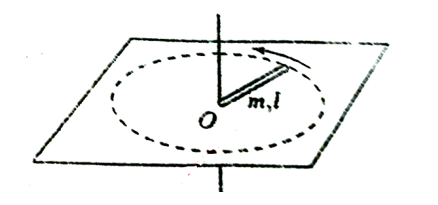
\includegraphics[width=0.4\textwidth]{2012_10.png}
		\caption{解答1 示意图}
	\end{flushright}
\end{figure}

\exercise{2}
设快速运动的介子的能量约为$E=3000$MeV,而这种介子在静止时的能量$E_0=100$MeV。若这种介子的固有寿命为$\tau_0=2\times 10^{-6}$s,试求:

\exercisequestion{1}介子衰变前运动的距离。

\vspace{10em}
\exercise{3}
电荷分布在半径为$R$的球体内,电荷量体密度为$\rho=\rho_0(1-\dfrac{r}{R})$,式中$\rho_0$为常量,$r$为球心到球内一点的距离,试求:

\exercisequestion{1}球内、球外的电场强度大小;

\exercisequestion{2}电场强度的最大值。

\vspace{10em}
\exercise{4}
如图所示,一无限长直导线$L_1$载有电流$I_1$,旁边有与它垂直且共面的一段导线$L_2$,$L_2$长为$l$,载有电流$I_2$,靠近$L_1$的一端到$L_1$的距离也是$l$,试求:

\exercisequestion{1}$L_1$上的电流作用在$L_2$上的力的大小及方向。
\begin{figure}[!h]
	\begin{flushright}
		\includegraphics[width=0.4\textwidth]{2012_11.ai}
		\caption{解答4 示意图}
	\end{flushright}
\end{figure}

\exercise{5}
两根无限长的平行输电线,相距为$l$,载有大小相等而方向相反的电流$I=I_0cos\omega t$ ;旁边有一长为$a$,宽为$b$的矩形线圈,它们在同一平面内,长边与输电线平行,到最近一条的距离为$d$,如图所示,试求:

\exercisequestion{1}导线与矩形线圈的互感系数;

\exercisequestion{2}矩形线圈中的感应电动势。
\begin{figure}[!h]
	\begin{flushright}
		\includegraphics[width=0.4\textwidth]{2012_12.ai}
		\caption{解答5 示意图}
	\end{flushright}
\end{figure}

\newpage
\section{参考答案}
\note 对于解析中没带矢量符号的矢量,认为是在计算其大小,以后不再说明。
\vspace{-2em}
\subsection{选择题和填空题}
\choosing{1}{10} CBBBD DADBA

\filling{\sqrt{mkx_0^2}}
{\dfrac{2}{7}g\quad\dfrac{2}{3}g}
{\text{减小\quad 增大\quad 不变\quad 增大}}
{\dfrac{1}{4}m_0c^2\quad \dfrac{\sqrt{3}}{2}c}
{\dfrac{q}{4\pi\varepsilon_0r^2}\quad\dfrac{q}{4\pi\varepsilon_0r_c}}
{\dfrac{\sigma}{2\varepsilon_0}\quad\dfrac{3\sigma}{2\varepsilon_0}\quad\dfrac{\sigma}{2\varepsilon_0}}
{\dfrac{\mu_0}{4\pi R}|I_1(2\pi-\theta)-I_2\theta|\quad 0}
{\dfrac{\sqrt{5}}{4}l\dy{B}{t}\quad\dfrac{1}{2}l^2\dy{B}{t}}

部分题目解析:

\exerciseanswer{选择}{4}

\tips 光的波长是与频率成反比的,二者之积为光速。不同颜色的光的波速相同。

\exerciseanswer{选择}{8}

\solve 设圆弧初始时电荷线密度为$\lambda$,则后来电荷线密度为$2\lambda$,半径为$R$,两种情况下均以O与圆弧中点连线为极轴,建立坐标系进行积分。
\begin{align*}
	E_0&=\int_{-\frac{1}{3}\pi}^{\frac{1}{3}\pi}\dfrac{1}{4\pi\varepsilon_0}\dfrac{\lambda R\di{\theta}}{R^2}\cos\theta\\
	&=\dfrac{\sqrt{3}\lambda}{4\pi\varepsilon_0R}\\
	E&=\int_{-\frac{1}{6}\pi}^{\frac{1}{6}\pi}\dfrac{1}{4\pi\varepsilon_0}\dfrac{2\lambda R\di{\theta}}{R^2}\cos\theta\\
	&=\dfrac{\lambda}{2\pi\varepsilon_0R}=\dfrac{2}{\sqrt{3}}E_0
\end{align*}
故选D。

\exerciseanswer{选择}{10}

\note A选项说法不准确。麦克斯韦把$\dy{\varPsi}{t}$称为$I_D$,前者的含义就是变化的电场,所以说位移电流就是变化电场的一个替代,为了使“电流生磁”的形式保持不变。若要用“产生”,说明二者应该是独立的两个事物,而事实上并不是。

\exerciseanswer{填空}{1}

\tips 本题综合了动能定理、动量定理、动能和动量的关系,由动能到动量再到冲量,计算简单但融入了较多思想,希望同学们理解、运用。

\exerciseanswer{填空}{2}

\solve 第一种情况,人和轻绳端点(右端物体)的加速度相同,故列式上与把人换成质量为$4m$的重物无异。由角动量定理:
\begin{gather*}
	(4mg-2mg)R=\dy{(4mRv+2mRv+Jw)}{t}=7mR^2\beta\\
	\beta=\dfrac{2}{7}g
\end{gather*}
第二种情况,人对轴的角动量不变,故:
\begin{gather*}
(4mg-2mg)R=\dy{(2mRv+Jw)}{t}=3mR^2\beta\\
\beta=\dfrac{2}{3}g
\end{gather*}

\exerciseanswer{填空}{5}

\tips 导线连接后,二者成为等势体,只考虑球壳外的场强即可。

\exerciseanswer{填空}{7}

\solve 本题是毕奥萨法尔定律的应用。由叉积的性质,两段直导线在$O$处的磁感应强度为0,而对圆导线:
\begin{align*}
	B_1&=\int_{0}^{2\pi-\theta}\dfrac{\mu_0}{4\pi}\dfrac{I_1\di{r}}{R}\\
	&=\dfrac{\mu_0I_1}{4\pi R}(2\pi-\theta)
\end{align*}
同理
\[
	B_2=\dfrac{\mu_0I_2}{4\pi R}\theta
\]
所以第一空应填$\dfrac{\mu_0}{4\pi R}|I_1(2\pi-\theta)-I_2\theta|$
由题,$I_1,I_2$流过的两段导线并联,而其电阻与长度成正比,电流与长度(其对应的圆心角)成反比,代入即得磁感应强度为零。

\exerciseanswer{填空}{8}

\solve 可以在磁场区内部取一半径为$r$的环路,其上每一点都有:
\begin{gather*}
	E_v\cdot 2\pi r=\dy{B}{t}\cdot \pi r^2\\
	E_v=\dfrac{r}{2}\dy{B}{t}
\end{gather*}
方向沿圆周切线。所以第一空填$\dfrac{\sqrt{5}}{4}l\dy{B}{t}$。

\begin{figure}
	\centering
	\includegraphics[width=0.4\textwidth]{2012_s1.ai}
\end{figure}
如图所示,第二空所求电动势无法在回路中研究,故对感生电场强度积分。
\begin{align*}
	\varepsilon_{\textrm{dc}}&=\int_{-\frac{l}{2}}^{\frac{l}{2}}E_v\cos\theta\di{x}\\
	&=\int_{-\frac{l}{2}}^{\frac{l}{2}}\dfrac{r}{2}\dy{B}{t}\cdot\dfrac{l}{r}\di{x}(r=\sqrt{x^2+l^2})\\
	&=\dfrac{1}{2}l^2\dy{B}{t}
\end{align*}

\subsection{解答题}
\solves{1}%普通格式,英文括号,然后空一下
(1)设细棒外侧端点为$A$。
\begin{align*}
	J&=\int_O^A\di{m\cdot r^2}\\
	&=\dfrac{m}{L}\int_0^Lx^2\di{x}\\
	&=\dfrac{1}{3}mL^2
\end{align*}
(2)
\begin{align*}
	M_f&=\int_O^A|\vec{r}\times\vec{F}|\\
	&=\int_0^Lx\cdot\mu\cdot\dfrac{m}{L}\di{x}g\\
	&=\dfrac{\mu mg}{L}\int_0^Lx\di{x}\\
	&=\dfrac{1}{2}\mu mgL
\end{align*}
方向与棒角动量方向相反(竖直向下)。

(3)
\begin{gather*}
	M_f=J\beta\\
	-\omega_0=0-\beta t
\end{gather*}
则
\[
	t=\dfrac{J\omega_0}{M_f}=\dfrac{2L\omega_0}{3\mu g}
\]

\solves{2}
由题:
\begin{gather*}
	E=mc^2=\dfrac{m_0}{\sqrt{1-{(\frac{v}{c})}^2}}\\
	E_0=m_0c^2
\end{gather*}
则:
\begin{gather*}
	\sqrt{1-{(\frac{v}{c})}^2}=\dfrac{E_0}{E}=\dfrac{1}{30}\\
	v=\dfrac{\sqrt{899}}{30}c
\end{gather*}
而
\[
	\tau=\dfrac{\tau_0}{\sqrt{1-{(\frac{v}{c})}^2}}=30\tau_0
\]
故:
\[
	s=v\tau=\sqrt{899}c\tau_0=1.799\times 10^4\textrm{m}
\]

\solves{3}
(1) 取球心与球体球心重合、半径为$r$的球面高斯面,由高斯定理:
\[
	E\cdot 4\pi r^2=\dfrac{q}{\varepsilon_0}
\]
在球内:
\begin{align*}
	q&=\int_0^r\rho_0(1-\dfrac{r}{R})\cdot 4\pi r^2\di{r}\\
	&=4\pi\rho_0\int_0^r(r^2-\dfrac{r^3}{R})\di{r}\\
	&=4\pi\rho_0(\dfrac{1}{3}r^3-\dfrac{1}{4R}r^4)
\end{align*}
在球外:
\begin{align*}
q&=\int_0^R\rho_0(1-\dfrac{r}{R})\cdot 4\pi r^2\di{r}\\
&=4\pi\rho_0\int_0^R(r^2-\dfrac{r^3}{R})\di{r}\\
&=\dfrac{1}{3}\pi\rho_0R^3
\end{align*}
所以$E=
\begin{cases}
\dfrac{\rho_0}{\varepsilon_0}(\dfrac{1}{3}r-\dfrac{1}{4R}r^2),&r<R\\
\dfrac{\rho_0R^3}{\varepsilon_0r^2},&r>R
\end{cases}$

(2) 由(1),$r>R$时,$E$随$r$的增大而减小;

$r<R$时,由二次函数性质,$r>\dfrac{2}{3}R$时,$E$随$r$的增大而减小,反之相反。

电场强度函数是连续的,所以
\[
	E_{max}=E(\dfrac{2}{3}R)=\dfrac{\rho_0R}{9\varepsilon_0}
\]

\solves{4}
对$I_1$的磁场,\amperecircuitaltheorem{1}
\begin{align*}
	F&=\int_l^{2l}|I\di{\vec{r}}\times \vec{B}|\\
	&=\dfrac{\mu_0I_1I_2}{2\pi}\int_l^{2l}\dfrac{\di{r}}{r}\\
	&=\dfrac{\mu_0I_1I_2\ln 2}{2\pi}
\end{align*}
方向:沿$I_1$的方向。

\solves{5}
(1) \amperecircuitaltheorem{}以垂直于纸面向内(沿线圈顺时针)为正向。
\begin{align*}
	\phi&=\phi_1+\phi_2\\
	&=\int_{d}^{b+d}\dfrac{\mu_0I}{2\pi r}\cdot a\di{r}
	-\int_{d+l}^{b+d+l}\dfrac{\mu_0I}{2\pi r}\cdot a\di{r}\\
	&=\dfrac{\mu_0Ia}{2\pi}(\int_{d}^{b+d}\dfrac{\di{r}}{r}-\int_{d+l}^{b+d+l}\dfrac{\di{r}}{r})\\
	&=\dfrac{\mu_0Ia}{2\pi}\ln\dfrac{(b+d)(d+l)}{d(b+d+l)}
\end{align*}
所以
\[
	M=\dfrac{\phi}{I}=\dfrac{\mu_0a}{2\pi}\ln\dfrac{(b+d)(d+l)}{d(b+d+l)}
\]
(2) 
\begin{align*}
	\varepsilon&=-\dy{\phi}{t}\\
	&=-\dfrac{\mu_0a}{2\pi}\ln\dfrac{(b+d)(d+l)}{d(b+d+l)}\cdot\dy{I}{t}\\
	&=\dfrac{\mu_0I_0a\omega}{2\pi}\ln\dfrac{(b+d)(d+l)}{d(b+d+l)}\sin\omega t
\end{align*}

\newpage
\chapter{2011年期末试题}
\section{选择题}
\exercise{1}
一枚在星际空间飞行的火箭,当它以恒定的速率燃烧燃料时,运动学方程为$x=ut+u(\dfrac{1}{b}-t)\ln(1-bt)$。其中$u$是喷出气流相对于火箭的喷射速度,是一个常量,$b$是与燃烧速率成正比的一个常量,则此火箭的速度与加速度的表达式分别为
\optionss{-u\ln(1-bt),\dfrac{-bu}{1-bt}}
{-u\ln(1-bt),\dfrac{bu}{1-bt}}
{u\ln(1-bt),\dfrac{-bu}{1-bt}}
{u\ln(1-bt),\dfrac{bu}{1-bt}}

\exercise{2}
一光滑的内表面半径为10cm的半球形碗。如图所示,以角速度$\omega$绕其对称轴OC旋转,已知放在碗内的一个小球P相对于碗静止,其位置高于碗底4cm,由此可推知碗的旋转角速度约为
\option{13\textrm{rad/s}}
{17\textrm{rad/s}}
{10\textrm{rad/s}}
{18\textrm{rad/s}}

\begin{figure}[!h]
	\centering
	\subfigure[选择2 示意图]{
		\begin{minipage}[t]{0.4\linewidth}
			\includegraphics[width=\textwidth]{2011_1.ai}
	\end{minipage}}
	\quad
	\subfigure[选择4 示意图]{
		\begin{minipage}[t]{0.4\linewidth}
			\includegraphics[width=\textwidth]{2011_2.ai}
	\end{minipage}}
	\caption{两张题图}
\end{figure}

\exercise{3}已知地球的质量为$m$,太阳的质量为$M$,地心与日心的距离为$R$,引力常量为$G$,则地球绕太阳做圆周运动的角动量为
\option{m\sqrt{GMR}}
{\sqrt{\dfrac{GMm}{R}}}
{m\sqrt{\dfrac{GM}{R}}}
{\sqrt{GMmR}}

\exercise{4}
一轻绳跨过一具有水平光滑轴,质量为$M$的定滑轮,绳的两端分别悬有质量为$m_1,m_2$的物体($m_1<m_2$),如图所示,绳与轮之间无相对滑动,分别考虑轮为实心和空心的情况,当$m_2$下降相同高度后获得的速率分别为$v_1$和$v_2$,试确定两者大小关系
\option{v_1=v_2}
{v_1<v_2}
{v_1>v_2}
{\text{无法确定}}

\exercise{5}
根据相对论力学,动能为0.25MeV的电子,其运动速度约等于(电子的静能为$m_0c^2$=0.5MeV,$c$为真空中光的速度)
\option{0.1c}
{0.5c}
{0.75c}
{0.85c}

\exercise{6}两个同心均匀带电球面,半径分别为$R_1,R_2(R_1<R_2)$所带电量分别为$Q_1,Q_2$,设某点与球心的距离为$r$,当$R_1<r<R_2$时,该点的电场强度的大小为
\optionss{\dfrac{1}{4\pi\varepsilon_0}\dfrac{Q_1+Q_2}{r^2}}
{\dfrac{1}{4\pi\varepsilon_0}\dfrac{Q_1-Q_2}{r^2}}
{\dfrac{1}{4\pi\varepsilon_0}(\dfrac{Q_1}{r^2}+\dfrac{Q_2}{R^2})}
{\dfrac{1}{4\pi\varepsilon_0}\dfrac{Q_1}{r^2}}

\exercise{7}
有一沿水平方向放置的带电直线,长为L,电荷线密度为$\lambda$,则带电直线右侧延长线上距离带电直线左端点为$r(r>L)$处的电势大小为
\optionss{\dfrac{\lambda}{4\pi\varepsilon_0}\ln\dfrac{r+L}{r}}
{\dfrac{\lambda}{4\pi\varepsilon_0}\ln\dfrac{r-L}{r}}
{\dfrac{\lambda}{4\pi\varepsilon_0}\ln\dfrac{L}{r+L}}
{\dfrac{\lambda}{4\pi\varepsilon_0}\ln\dfrac{L}{r-L}}

\exercise{8}
将一空气平行板电容器接到电源上,充电到一定电压后,在保持与电源连接的情况下,再将一块与平板面积相同的金属板平行的插入两极板间,金属板的插入及所处位置不同,对电容器储存电能的影响为:
\options    
{储能减少,但与金属板的位置无关}
{储能减少,且与金属板的位置有关}
{储能增加,但与金属板的位置无关}    
{储能增加,且与金属板的位置有关}

\begin{figure}[!h]
	\centering
	\subfigure[选择8 示意图]{
		\begin{minipage}[t]{0.3\linewidth}
			\includegraphics[width=\textwidth]{2011_3.ai}
	\end{minipage}}
	\quad
	\subfigure[选择9 示意图]{
		\begin{minipage}[t]{0.3\linewidth}
			\includegraphics[width=\textwidth]{2011_4.ai}
	\end{minipage}}
	\quad
	\subfigure[选择10 示意图]{
		\begin{minipage}[t]{0.3\linewidth}
			\includegraphics[width=\textwidth]{2011_5.ai}
	\end{minipage}}
	\caption{三张题图}
\end{figure}

\exercise{9}
如图所示,一长直导线中部弯成半径为$r$的半圆形,导线中通以恒定电流$I_1$,则弧心O点处的磁感应强度的大小和方向分别是
\optionss{\dfrac{\mu_0I}{2\pi r}+\dfrac{\mu_0I}{4r}\text{,向外}}
{\dfrac{\mu_0I}{2\pi r}+\dfrac{\mu_0I}{4r}\text{,向里}}
{\dfrac{\mu_0I}{4r}\text{,向外}}
{\dfrac{\mu_0I}{4r}\text{,向里}}

\exercise{10}
在圆柱形空间内有一磁感应强度为$B$的均匀磁场垂直于纸面向里,$B$的大小以恒定速率变化,有一长度为$L$的金属棒先后放在磁场的不同位置,位置1$(a,b)$感应电动势大小为$\varepsilon_1$,位置2$(a',b')$感应电动势大小为$\varepsilon_2$,如图所示,则
\optionss{\varepsilon_1=\varepsilon_2\neq0}
{\varepsilon_1<\varepsilon_2}
{\varepsilon_1>\varepsilon_2}
{\varepsilon_1=\varepsilon_2=0}

\section{填空题}

\exercise{1}
质点沿半径为$R$的圆做圆周运动,某一时刻其加速度大小为$a$,方向与位矢的夹角为$\theta$,则该时刻质点的速率为\ul,切向加速度的大小为\ul。

\exercise{2}
质量为$m$=1kg的质点,从静止出发,在水平面内沿x轴正向运动。其所受合力方向与运动方向相同,合力大小为$F=3+2x$,物体在开始运动的3m内合力做功$A=$\ul;$x=3$时,其速率$v=$\ul。

\exercise{3}
长为$L$,质量为$M$的均匀细杆,以及一长为$L$,质量为$M$的单摆(绳的质量忽略不计),今用同样的弹丸(质量均为$m$)以同样的速度$v$沿水平方向分别击中杆和单摆的下端,并与之合为一体,则击中后的瞬间杆的角速度为\ul,单摆的角速度为\ul。

\exercise{4}
如图所示,图中实线为某电场的电场线,虚线为等势面,则$E_A,E_B,E_C$的大小关系为\ul,$U_A,U_B,U_C$的大小关系为\ul。


\begin{figure}[!h]
	\centering
	\subfigure[填空4 示意图]{
		\begin{minipage}[t]{0.4\linewidth}
			\includegraphics[width=\textwidth]{2011_6.ai}
	\end{minipage}}
	\quad
	\subfigure[填空5 示意图]{
		\begin{minipage}[t]{0.4\linewidth}
			\includegraphics[width=\textwidth]{2011_7.ai}
	\end{minipage}}
	\caption{两张题图}
\end{figure}

\exercise{5}
A、B为真空中两个平行的无限大均匀带电平面,平面间的电场强度大小为$E_0$,$B$平面外侧的电场强度为$\dfrac{E_0}{3}$,方向由A指向B,则A、B平面的电荷密度分别为$\sigma_1=$\ul,$\sigma_2=$\ul。

\exercise{6}
一个通有电流$I$的导体,厚度为$D$,横截面积为$S$,放在磁感应强度为$B$的匀强磁场(磁感应强度为 $B$)中,磁场方向垂直于导体的侧平面,现测得导体上下两面电势差为$V$,此导体的霍尔系数为\ul。

\exercise{7}
如图所示,在无限长直载流导线的右侧有面积为$S_1,S_2$的两个矩形回路,两个回路和长直载流导线在同一平面内,且电流方向和矩形回路的一边平行,则通过面积为$S_1$的矩形回路的磁通量和通过面积为$S_2$的矩形回路的磁通量之比为\ul。

\begin{figure}[!h]
	\centering
	\subfigure[填空7 示意图]{
		\begin{minipage}[t]{0.4\linewidth}
			\includegraphics[width=\textwidth]{2011_8.ai}
	\end{minipage}}
	\quad
	\subfigure[填空8 示意图]{
		\begin{minipage}[t]{0.4\linewidth}
			\includegraphics[width=\textwidth]{2011_9.ai}
	\end{minipage}}
	\caption{两张题图}
\end{figure}

\exercise{8}
一无铁芯的长直密绕螺线管,在保持半径和总匝数不变的情况下,把螺线管稍微拉长一点,不考虑漏磁的理想情况下,则它的自感系数将\ul(变大,变小或不变)。


\section{解答题}%用\vspace控制答题空间
%\begin{wrapfigure}{1}[r][1em]\end{wrapfigure}
\exercise{1}
如图所示,一个转动惯量为$J$,半径为$R$的定滑轮上面绕有细绳,并沿水平方向拉着一个质量为$M$的物体A,整个装置静止且细绳处于拉直状态。现有一质量为$m$的子弹在距转轴$\frac{R}{2}$处。试求:

\exercisequestion{1}求子弹射入并停留在滑轮边缘后,滑轮开始转动的角速度 。

\exercisequestion{2}如果定滑轮拖着A刚好转动一周停止,求A与地面的摩擦系数。(轴上摩擦力忽略不计);

\begin{figure}
	\begin{flushright}
		\includegraphics[width=0.4\textwidth]{2011_10.ai}
		\caption{解答1 示意图}
	\end{flushright}
\end{figure}

\exercise{2}
在6000m的高空大气层产生了一个$\pi$介子,以速度$v=0.998c$飞向地球,假定该$\pi$介子在其自身的静止系中的寿命约等于其平均寿命$2\times 10^{-6}$,试从下面两个角度,即地球上的观察者和介子静止系中观察者,来判断该介子能否到达地球。

\exercise{3}
一半径为$R$的无限长带电圆柱,其电荷体密度$\rho=\rho_0r(r<R)$,$\rho_0$为常量,求电场强度分布。

\exercise{4}
半径为$R$的无限长带电圆柱导体,通有电流$I$,$I$均匀分布在其横截面上。

\exercisequestion{1}试求外的磁感应强度$B$的分布。

\exercisequestion{2}在柱体内挖一个空心圆柱,空心部分的半径为$b$,轴线与圆柱轴线平行但不重合,两者相距为$a$。若此时圆柱体内电流为$I$,均匀分布在其横截表面上,试求圆柱轴线和空心圆柱轴线上的磁感应强度$B$的大小。

\exercise{5}
有一根辐条的轮子在均匀磁场中转动,转动轴与磁感应强度$B$平行,如图所示,轮子和辐条都是导体,辐条长为$R$,轮子每秒转$N$圈。两条导线a和b通过各自的电刷分别和轮轴和轮缘接触。

\exercisequestion{1}试求a,b间的感应电动势$\varepsilon_1$;

\exercisequestion{2}若在a,b间接一个电阻使辐条中的电流为$I$,试问$I$的方向如何?

\exercisequestion{3}试求这时磁场作用在辐条上的力对轮轴的力矩$M$的大小。
\begin{figure}[!h]
	\begin{flushright}
		\includegraphics[width=0.4\textwidth]{2011_11.ai}
		\caption{解答5 示意图}
	\end{flushright}
\end{figure}

\newpage
\section{参考答案}
\subsection{选择题和填空题}
\choosing{1}{10} BAACC DDCCC

\filling{\sqrt{aR|\cos\theta|}\quad a\sin\theta}
{18\textrm{J}\quad6\textrm{m/s}}
{\dfrac{mv}{(m+\frac{1}{3}M)L}\quad\dfrac{mv}{(m+M)L}}
{E_A<E_B<E_C\quad U_A>U_B>U_C}
{\dfrac{4}{3}\varepsilon_0E_0\quad -\dfrac{2}{3}\varepsilon_0E_0}
{\dfrac{VD}{IB}}
{1(1:1)}
{\textrm{变小}}

部分题目解析:

\exerciseanswer{选择}{4}

\tips 两种情况的区别在于,实心轮质量分布靠近轮心,转动惯量较小,加速度大。

\exerciseanswer{选择}{9}

\tips 由毕奥—萨法尔定律,直径部分在O点产生的磁感应强度为零。不可与无线长直导线模型混淆,认为磁感应强度是无穷。

\exerciseanswer{选择}{10}

\solve 均匀变化磁场产生的感应电动势有两种求解方法:

(1) 感生电场叠加。这是普适的方法,往往需要投影、积分,可能较麻烦。常用于计算一段导体上的电动势。在本题中,设导线中心到O的距离为$d$,则:
\begin{align*}
\varepsilon&=\int_{-\frac{1}{2}L}^{\frac{1}{2}L}\left|\dy{B}{t}\right|\cdot\dfrac{\sqrt{x^2+d^2}}{2}\cdot\dfrac{d}{\sqrt{x^2+d^2}}\di{x}\\
&=\left|\dy{B}{t}\right|\cdot\dfrac{Ld}{2}
\end{align*}
可见$\varepsilon$与$d$成正比,故选C。

(2) 法拉第电磁感应定律法。此法可计算环路、一段导体的电动势,只要面积容易计算。感生电场方向垂直于相应半径,故任意场点与O的连线上电动势为零,则一段导体的电动势等于相应环路的电动势。本题中:
\begin{align*}
\left|\varepsilon\right|&=\left|\dy{\phi}{t}\right|\\
&=\left|\dy{B}{t}\right|S\\
&=\left|\dy{B}{t}\right|\cdot\dfrac{Ld}{2}
\end{align*}
这样相对更容易计算。

\exerciseanswer{填空}{5}
由无限带电平面场强公式$E=\dfrac{\delta}{2\varepsilon_0}$得(向右为正向):
\begin{align*}
\dfrac{\delta_1}{2\varepsilon_0}-\dfrac{\delta_2}{2\varepsilon_0}&=E_0\text{(平面间)}\\
\dfrac{\delta_1}{2\varepsilon_0}+\dfrac{\delta_2}{2\varepsilon_0}&=\dfrac{E_0}{3}\text{(B
	平面右侧)}
\end{align*}
解得:
\begin{gather*}
\delta_1=\dfrac{4}{3}\varepsilon_0E_0\\
\delta_2=-\dfrac{2}{3}\varepsilon_0E_0
\end{gather*}


\exerciseanswer{填空}{8}%查书页码、版本、具体叙述

\solve
参照大学物理课本(黑皮)第……页的推导,计算公式为$L_0=\mu_0n^2V=\mu_0S\dfrac{N^2}{l}$,其中$n$是单位长度上的匝数,$N$是总匝数,$S$是横截面积,$l$是螺线管长度,按此分析,答案应是减小。该模型针对的是无限长螺线管,且认为半径很小,管内磁感应强度处处相等,这里并不完全严谨。(我回去再看看书)

感兴趣的同学可以参考相关文献,如邰爱东给出了两种准确的计算方法\footnote{邰爱东.有限长直密绕螺线管的自感系数[J].物理与工程,2003(06):8-9.}。


\subsection{解答题}
\solves{1}%普通格式,英文括号,然后空一下
(1) 射入时,由角动量守恒:
\begin{gather*}
R\cdot mv_0\sin\dfrac{5\pi}{6}=J\omega+mR^2\omega+MR^2\omega\\
\omega=\dfrac{mv_0R}{2(J+mR^2+MR^2)}
\end{gather*}
(2) 由动能定理:
\begin{gather*}
-\dfrac{1}{2}(J+mR^2+MR^2)\omega^2=-\mu Mg\cdot 2\pi R\\
\mu=\dfrac{m^2v_0^2R}{16\pi Mg(J+mR^2+MR^2)}
\end{gather*}

\solves{2}
对地球上的观察者:
\begin{gather*}
\tau=\dfrac{\tau_0}{\sqrt{1-{\left(\frac{v}{c}\right)}^2}}=\dfrac{2\times 10^{-6}}{\sqrt{1-0.998^2}}=3.16\times 10^{-5}(\textrm{s})\\
t=\dfrac{s_0}{v}=\dfrac{6000}{0.998c}=2.00\times 10^{-5}(\textrm{s})<\tau
\end{gather*}
故能到达地球。

对$\pi$介子系观察者:
\begin{align*}
s&=s_0\sqrt{1-{\left(\frac{v}{c}\right)}^2}\\
t'&=\dfrac{s}{v}=\dfrac{s_0}{v}\sqrt{1-{\left(\frac{v}{c}\right)}^2}\\
&=2.00\times 10^{-5}\times 0.0632\\
&=1.27\times 10^{-6}(\textrm{s})<\tau_0
\end{align*}
故能到达地球。

\solves{3}
取半径为$r$、高为$h$的高斯面,由高斯定理:

$r<R$时,
\begin{gather*}
E\cdot 2\pi rh=\dfrac{1}{\varepsilon_0}\int_0^r \rho\cdot 2\pi rh\di{r}=\dfrac{2\pi h\rho_0}{\varepsilon_0}\int_0^rr^2\di{r}\\
E=\dfrac{\rho_0r^2}{3\varepsilon_0}
\end{gather*}
$r>R$时,
\begin{gather*}
E\cdot 2\pi rh=\dfrac{1}{\varepsilon_0}\int_0^R \rho\cdot 2\pi rh\di{r}=\dfrac{2\pi h\rho_0}{\varepsilon_0}\int_0^Rr^2\di{r}\\
E=\dfrac{\rho_0R^3}{3\varepsilon_0r}
\end{gather*}
\therefore$E=$
$\begin{cases}
\vspace{0.3em}%不会调cases的行距。。
\dfrac{\rho_0r^2}{3\varepsilon_0},&r<R\\
\vspace{0.2em}
\dfrac{\rho_0R^3}{3\varepsilon_0r},&r>R
\end{cases}$
,方向沿场点处高斯面的法向量向外。

\note 这种求分布的题最好还是写上方向。

\solves{4}
(1) 在距离导体中心$r$处,取一半径为$r$的环路,由安培环路定理:

$r<R$时,
\begin{gather*}
B\cdot 2\pi r=\mu_0\dfrac{I}{\pi R^2}\cdot\pi r^2\\
B=\dfrac{\mu_0Ir}{2\pi R^2}
\end{gather*}
$r>R$时,
\begin{gather*}
B\cdot 2\pi r=\mu_0I\\
B=\dfrac{\mu_0I}{2\pi r}
\end{gather*}
\therefore$B=
\begin{cases}
\vspace{0.3em}
\dfrac{\mu_0Ir}{2\pi R^2},&r<R\\
\vspace{0.2em}
\dfrac{\mu_0I}{2\pi r},&r>R
\end{cases}$

方向沿该点处环路的切向量,与电流方向符合右手定则。

(2) 此时,电流面密度$\sigma=\dfrac{I}{\pi R^2-\pi b^2}$。%求调行距。。

该系统可看做半径为$R$、电流面密度为$\sigma$的圆柱和半径为$b$、电流面密度为$-\sigma$的圆柱的组合。
且它们在自己轴线上产生的磁感应强度为0。那么由(1):
\begin{figure}
	\centering
	\includegraphics[width=0.9\textwidth]{2011_s1.ai}
	\caption{解答4 解析示意图}
\end{figure}
对于圆柱轴线,$a>b$时,如左图:
\[
B_1=\left|\dfrac{-\mu_0\sigma\cdot\pi b^2}{2\pi a}\right|=\dfrac{\mu_0Ib^2}{2\pi a(R^2-b^2)}
\]
$a<b$时,如右图:
\[
B_1=\left|\dfrac{-\mu_0\sigma\cdot\pi a^2}{2\pi a}\right|=\dfrac{\mu_0Ia}{2\pi(R^2-b^2)}
\]
对于空心圆柱轴线,
\[
B_2=\dfrac{\mu_0\sigma\cdot\pi a^2}{2\pi a}=\dfrac{\mu_0Ia}{2\pi(R^2-b^2)}
\]
综上,$\cdots$

\solves{5}
(1) 
\begin{align*}
\varepsilon_1&=\int_{a}^{b}(\vec{v}\times\vec{B})\cdot\di{l}\\
&=\int_{0}^{R}l\omega B\di{l}\\
&=\dfrac{1}{2}BR^2\omega\\
&=\pi NBR^2
\end{align*}
(2) (电动势方向是从轮子中心到轮子外侧,所以电流方向为)$b\rightarrow a$.

(3)
\begin{align*}
M&=\int_{a}^{b}\left|\vec{l}\times(I\di{\vec{l}}\times\vec{B})\right|\\
&=BI\int_{0}^{R}l\di{l}\\
&=\dfrac{1}{2}BIR^2
\end{align*}
\newpage



\end{document}